\subsection{Data}

\begin{frame}{Visualizations are (mostly) evaluated on equivariance}
    \begin{description}
        \item[Expressiveness] structure preserving mappings from data to graphic (Mackinlay \cite{mackinlayAutomatingDesignGraphical1986})
        \item[Effectiveness] design choices made in deference to perceptual saliency (Mackinlay \cite{clevelandResearchStatisticalGraphics1987,clevelandGraphicalPerceptionTheory1984,chambersGraphicalMethodsData1983a, munznerVisualizationAnalysisDesign2014})
        \item[Naturalness] easier to understand when properties match (Norman \cite{norman_things_smart})
        \item[Graphical Integrity] graphs show \textbf{only} the data (Tufte \cite{tufteVisualDisplayQuantitative2001})
    \end{description}
\end{frame}


\begin{frame}{Visualization is commutative maps}

    \pause
    %% deconstruct D\R\V
    \begin{center}
        \textbf{Tam: Add topology and make it functional}
    \end{center}
\end{frame}

\begin{frame}{Models describe composition}
    \begin{description}
        \item[language model] APT, GoG: syntax, semantics, and grammar of graphics (Mackinlay, Wilkenson  \cite{mackinlayAutomatingDesignGraphical1986, mackinlayAUTOMATICDESIGNGRAPHICAL1987,wilkinsonGrammarGraphics2005})
        \item[functional dependencies] constrained maps between data and visual representation(Sugibuchi \cite{sugibuchiFramwork2009}) 
        \item[category theory] the semiotics of visualization are commutative (Vickers \cite{vickersUnderstandingViz2013})
        \item[algebraic process] data ($\alpha$) and viz ($\omega$) transforms are symmetric (Kindlmann and Scheidegger \cite{kindlmannAlgebraicProcessVisualization2014})
        \begin{columns}
            \column{.5\textwidth}
       
            \begin{description}
                \item[D] data 
                \item[R] representations
                \item[V] visualizations
            \end{description}
            \column{.5\textwidth}
            \begin{equation*}
                \begin{tikzcd}[ampersand replacement=\&]
                    D \arrow[d, "\alpha"'] \arrow[r, "r_1"] \& R \arrow[r, "\nu"]  \& V \arrow[d, "\omega"] \\
                    D \arrow[r, "r_2"']                     \& R \arrow[r, "\nu"'] \& V                    
                \end{tikzcd}
                \end{equation*}
       
        \end{columns} 
     
    \end{description}
\end{frame}


\begin{frame}{Mathematical Frameworks for evaluating visualization}
    \begin{enumerate}
        \item APT: visualization has syntax and semantics like a language  (Mackinlay  \cite{mackinlayAutomatingDesignGraphical1986, mackinlayAUTOMATICDESIGNGRAPHICAL1987})
        \item visualization has functional dependencies that can be represented as graphs (Sugibuchi \cite{sugibuchiFramwork2009}) 
        \item the semiotics of visualization are commutative in a category theory framework (Vickers \cite{vickersUnderstandingViz2013})
        \item data ($\alpha$) and viz ($\omega$) symmetries (Kindlmann and Scheidegger \cite{kindlmann2014algebraic})
        \begin{block}{$v\circ r_2 \circ \alpha =\omega\circ v\circ r_1$}
            \begin{equation*}
            \begin{tikzcd}[ampersand replacement=\&]
                D \arrow[d, "\alpha"'] \arrow[r, "r_1"] \& R \arrow[r, "\nu"]  \& V \arrow[d, "\omega"] \\
                D \arrow[r, "r_2"']                     \& R \arrow[r, "\nu"'] \& V                    
            \end{tikzcd}
            \end{equation*}
        \end{block}
\end{frame}


\begin{frame}{Structure is encoded in variables and continuity}
    \begin{figure}
        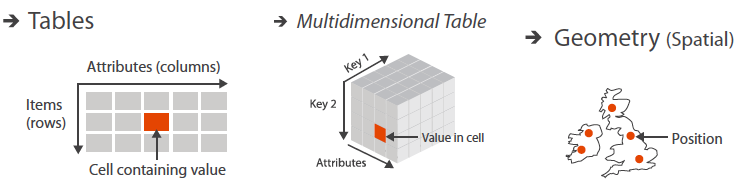
\includegraphics[width=1\textwidth]{figures/intro/munzner_datatypes.png}
        \caption{Image is figure 2.8 in Munzner's Visualization Analysis and Design\cite{munznerVisualizationAnalysisDesign2014}}
    \end{figure}
    \begin{description}
        \item[binding] metadata are structural \textit{keys} with associated \textit{values} (Munzner \cite{munznerVisualizationAnalysisDesign2014})] 
        \item[continuity])
        \item[variables] Fibers can hold schema like encodings of variables (Spivak \cite{spivakDatabasesAreCategories2010,spivakSIMPLICIALDATABASES})
    \end{description}
\end{frame}


begin{frame}{Monoid Actions: Permutation}
    \begin{figure}
        \includegraphics[width=1\linewidth]{figures/math/monoid_emoji.png}
    \end{figure}
\end{frame}

\begin{frame}{Why monoids? partial orders}
    \begin{figure}
        \begin{overprint}
            \onslide<1|handout:0>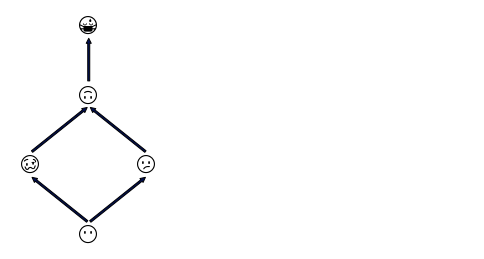
\includegraphics[width=1\linewidth]{figures/math/monoid_hasse.png}
            \onslide<2|handout:0>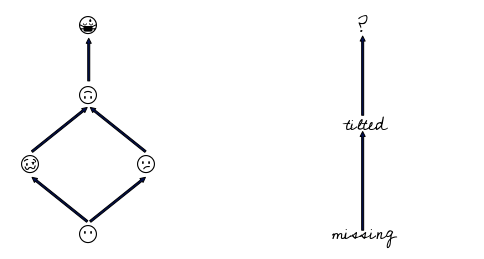
\includegraphics[width=1\linewidth]{figures/math/monoid_monotone.png}
            \onslide<3>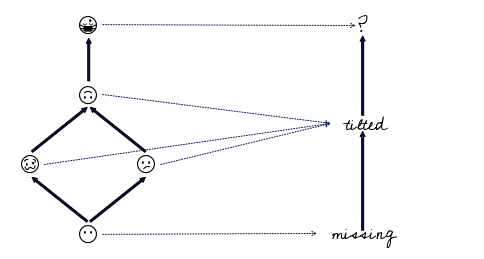
\includegraphics[width=1\linewidth]{figures/math/monoid_maps.png}
        \end{overprint}
    \caption{Inspired by definition 1.59 diagram in Spivak and Fong's An Invitation to Applied Category Theory \cite{fongInvitationAppliedCategory2019}}
    \end{figure}
\end{frame}

%appendix 
\begin{frame}{\dbase\ is an indexing space independent of component semantics}
    \begin{equation}
        \pi:\dtotal_1\oplus\ldots\oplus \dtotal_i \oplus\ldots \oplus \dtotal_n \rightarrow \dbase
    \end{equation}
\end{frame}




%rename so everything is consistent

\begin{frame}{MayaVI}
    \begin{figure}
        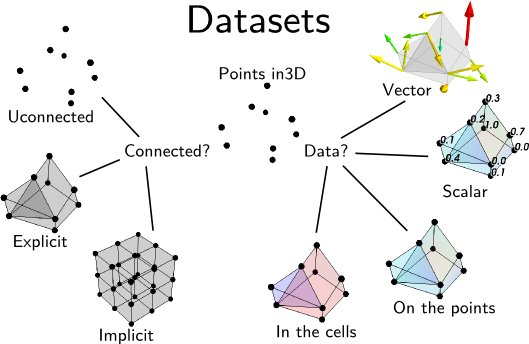
\includegraphics[height=.5\textheight]{figures/intro/dataset_diagram.png}
        \caption{Data Representation, MayaVi 4.7.2 docs\cite{DataRepresentationMayavi}}
    \end{figure}
\end{frame}

\begin{equation}
    \begin{equation*}
        \sheafc_{\dbasec, \dtotalc} \textcolor{artist}{\xrightarrow{\vartistc}} \sheafc_{\gbasec, \gtotalc}
    \end{equation*}
    \begin{equation*}
         (\sheafc_{\dbasec,\dtotalc} \textcolor{functor}{\xmapsto{\vindexpullc}} \vindexpullc \sheafc_{\dbasec,\dtotalc}) \textcolor{artist}{\xRightarrow{\vartistc_{\opensetgc}}} \sheafc_{\gbasec, \gtotalc} \tag{$\vartistc_{\opensetgc} \circ \vindexpullc = \vartistc$}
    \end{equation*}
    \begin{equation*}
        (\sheafc_{\dbasec,\dtotalc} \textcolor{artist}{\xRightarrow{\vartistc}} \sheafc_{\gbasec, \gtotalc}) \textcolor{functor}{\xmapsto{\vindexpushc}} \vindexpushc \sheafc_{\gbasec, \gtotalc} \tag{$\vindexpushc \circ \vartistc = \vartistc_{\opensetc}$}      
    \end{equation*}
    \begin{equation*}
        ((\sheafc_{\dbasec,\dtotalc} \textcolor{functor}{\xmapsto{\vindexpullc}} \vindexpullc \sheafc_{\dbasec,\dtotalc}) \textcolor{artist}{\xRightarrow{\vartistc_{\opensetgc}}} \sheafc_{\gbasec, \gtotalc})\textcolor{functor}{\xmapsto{\vindexpushc}} \vindexpushc \sheafc_{\gbasec, \gtotalc} \tag{$\vindexpushc \circ \vartistc_{\opensetgc} \circ \vindexpullc = \vartistc_{\opensetc}$}
    \end{equation*}
\end{equation}




    \begin{alertblock}
        \begin{align*}
            \vartistc(\dsectionc^{a}) = \vartistc(\dsectionc^{b}) &\centernot\implies \dsectionc^a = \dsectionc^b \\
            \vartistc(\dsectionc^{a})  = \vartistc(\dsectionc^{b}) &\implies \vartistc(\dfuncc_{\dtotalc}(\dsectionc^{a})) = \vartistc(\dfuncc_{\dtotalc}(\dsectionc^{b}))
        \end{align*}
    \end{alertblock}

    
\begin{frame}{Scatter: $\vmark(xpos, ypos)(\alpha, \beta)$}
    \begin{figure}[H]
        \begin{overprint}
            \onslide<1|handout:0>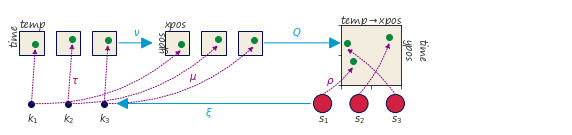
\includegraphics[width=1\linewidth]{figures/math/scatter_q.png}
            \onslide<2|handout:0>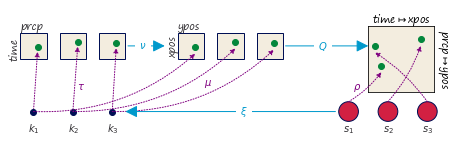
\includegraphics[width=1\linewidth]{figures/math/scatter_with_s.png}
        \end{overprint}
    \end{figure}   
\end{frame}

\begin{frame}{Line: $\vmark(xpos, \hat{n_{1}}, ypos, \hat{n_{2}})(\alpha, \beta)$ }
    \begin{figure}[H]
        \begin{overprint}
            \onslide<1|handout:0>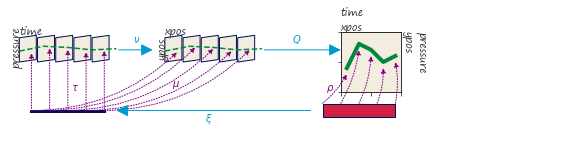
\includegraphics[width=1\linewidth]{figures/math/line_q.png}
            \onslide<2|handout:0>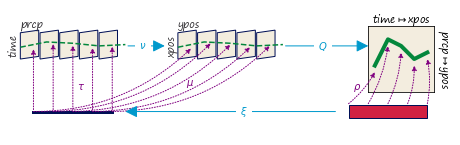
\includegraphics[width=1\linewidth]{figures/math/line_with_s.png}
        \end{overprint}
    \end{figure}   
\end{frame}

\begin{frame}{Image $\vmark(xpos, ypos, color)$}
    \begin{figure}[H]
        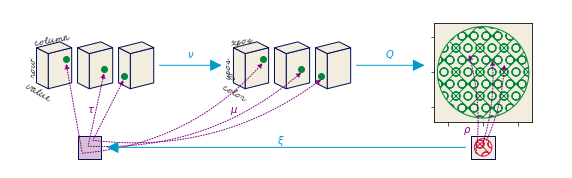
\includegraphics[width=1\textwidth]{figures/math/image.png}
    \end{figure}
\end{frame}

\begin{frame}{Build \vmark\ over \dbase: \vmarkd}
\begin{figure}[H]
    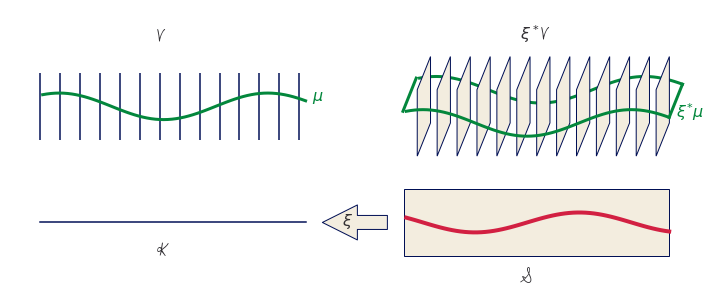
\includegraphics[width=1\textwidth]{figures/math/q_hat.png}
\end{figure}
\begin{equation*}\label{eq:qhat_q_s}
    \vmarkd(\vsection(\dbasepoint))(\gbasepoint) \coloneqq \vmark((\vsectionpull)(\gbasepoint))
\end{equation*} 
\end{frame}

\begin{frame}{Composition of artists $+ \coloneqq \sqcup \dtotal_{i}$} 
    \begin{figure}
        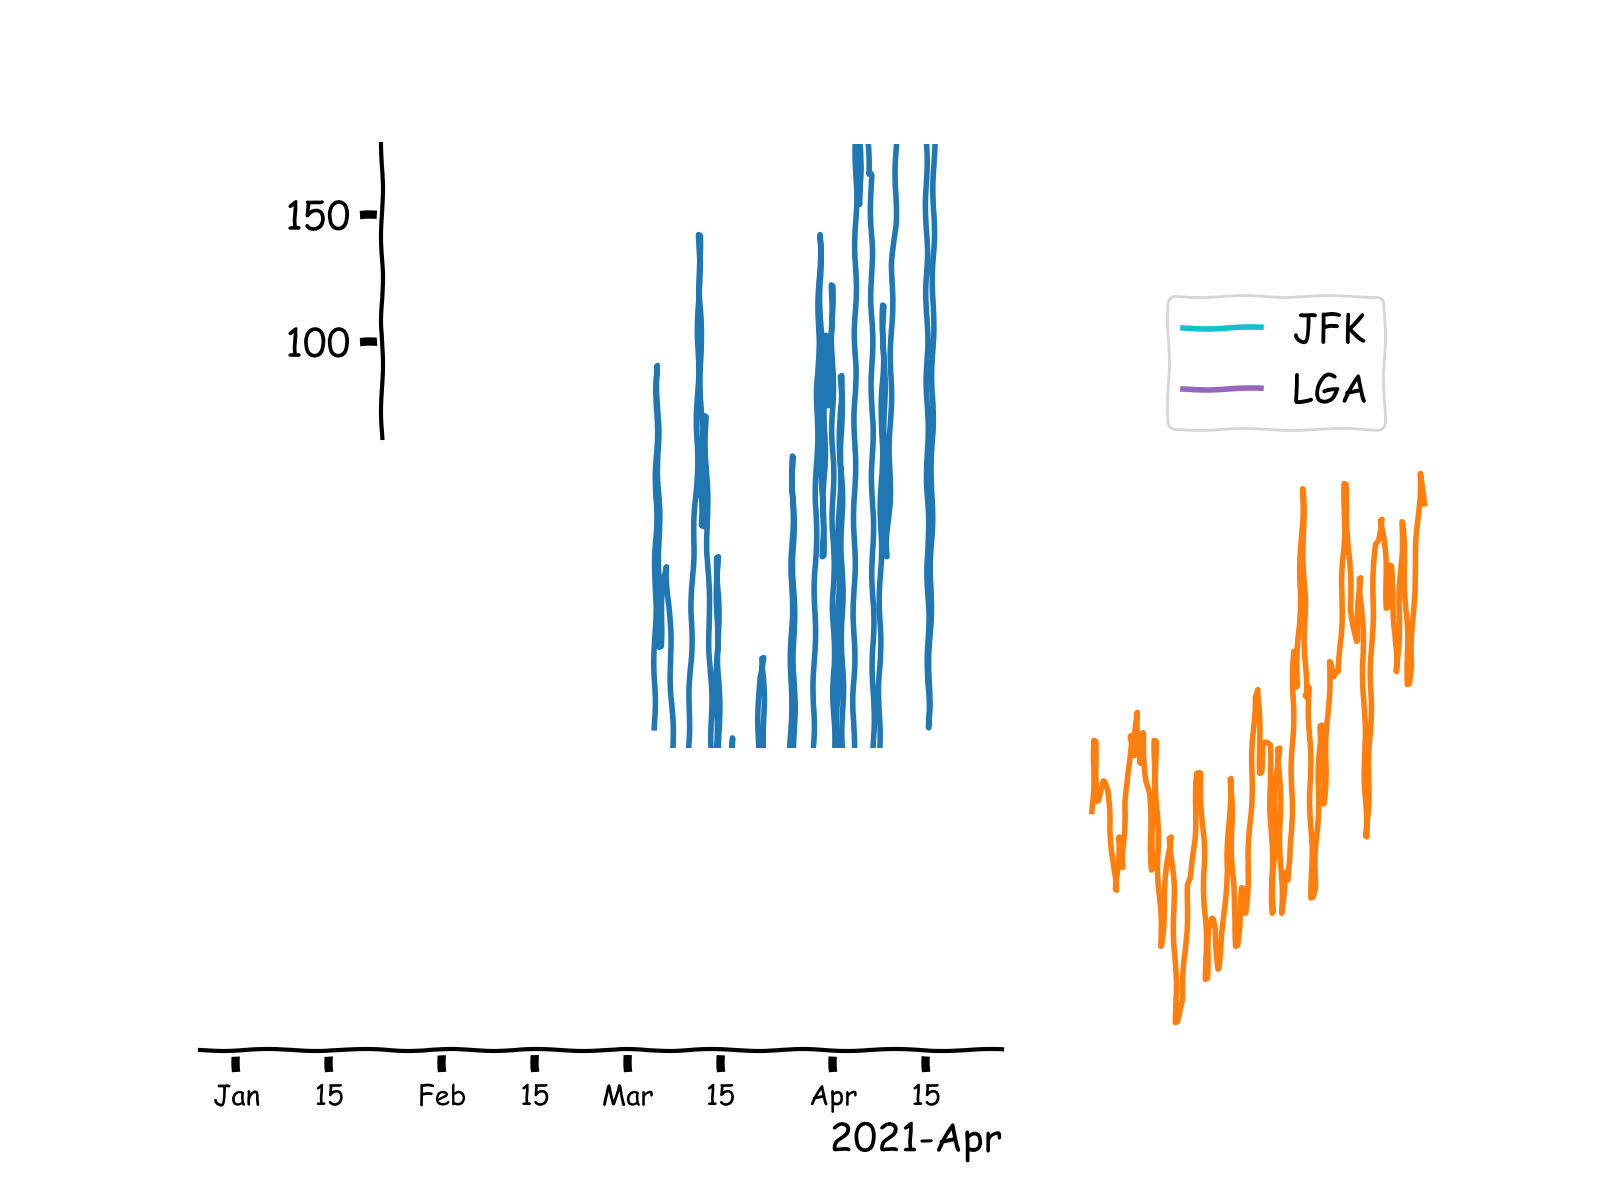
\includegraphics[width=1\textwidth]{figures/math/exploding_artist.png}
    \end{figure}
\end{frame}

\section{Code}
\begin{frame}{TEAM driven rearchitecture of Matplotlib}
    \begin{itemize}
        \item complex visualizations
        \pause 
        \item structure preserving maps from data to visual
        \begin{itemize}
            \item data and graphics have equivalent continuity
            \item properties are equivariant under monoid actions
        \end{itemize}  
        \pause
        \item fiber bundles are an abstraction
        \begin{itemize}
            \item topologically complex heterogenous data 
            \item target display spaces
        \end{itemize}
    \end{itemize}
\end{frame}

\begin{frame}[fragile]{How do we make things?}
    \begin{figure}[H]
        \begin{subfigure}{0.49\textwidth}
            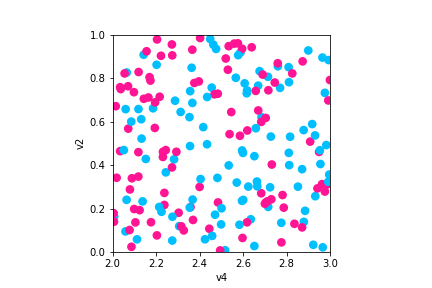
\includegraphics[width=\textwidth]{figures/code/scatter_0.png}
        \end{subfigure}
        \begin{subfigure}{0.49\textwidth}
            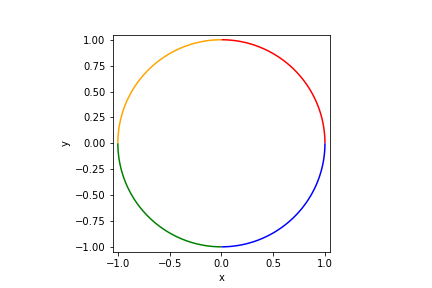
\includegraphics[width=\textwidth]{figures/code/line_1.png}
        \end{subfigure}
    \end{figure}
    \begin{columns}
    \column{0.49\textwidth}
    \begin{minted}{python}
    fig, ax = plt.subplots()
    artist = Point(data, transforms)
    ax.add_artist(artist)
    \end{minted}
    \column{.49\textwidth}
    \begin{minted}{python}
    fig, ax = plt.subplots()
    artist = Line(data, transforms)
    ax.add_artist(artist)
    \end{minted}
    \end{columns}
\end{frame}

\subsection{Artist}
\begin{frame}[fragile]{ \vchannel}
    \begin{minted}{python}
    cmap =  color.Categorical({'true':'deeppink', 'false':'deepskyblue'})
    transforms = {'x': {'name': 'v4', 'encoder': lambda x: x},
                    'y': {'name': 'v2', 'encoder': lambda x: x},
                    'facecolors': {'name':'v3', 'encoder': cmap}, 
                    's':{'name': None , 
                        'encoder': lambda _: itertools.repeat(.02)}}
    \end{minted}
    \begin{itemize}
        \item \mintinline{python}{lambda x: x} is identity \vchannel\
        \item \mintinline{python}|{'name':None}| map into \vfiber\ without corresponding \dsection\
        \item \mintinline{python}{color.Categorical} is custom \vchannel
    \end{itemize}
\end{frame}
    
\begin{frame}[fragile]{\vartist} %% rewrite w/ letters in talk
    \begin{minted}{python}
        class ArtistClass(matplotlib.artist.Artist):
            def __init__(self, E, V, *args, **kwargs):
                # set properties that are specific to the artist
                # stash the input E and V
                super().__init__(*args, **kwargs)
        
            def qhat(self, **args):
                # set the properties of the graphic
        
            def draw(self, renderer):
                # returns tau, indexed on fiber then key 
                tau = self.E.view(self.axes) 
                # visual channel encoding applied fiberwise 
                visual = {p_i: nu_i(tau_i)
                          for p_i, nu_i, tau)i 
                          in zip(self.V, tau)}
                self.qhat(**visual)
                # pass configurations off to the renderer
                super().draw(renderer)
        \end{minted}
\end{frame}

\begin{frame}[fragile]{\vmarkd}
\begin{minted}{python}
    class Point(mcollections.Collection):
        def assemble(self, x, y, s, facecolors='C0' ):
            # construct geometries of the circle glyphs in visual coordinates
            # set attributes of glyphs

    class Line(mcollections.LineCollection):
        def assemble(self, x, y, color='C0'):
            # assemble line marks as set of segments 
    \end{minted}
\end{frame}

\subsection{Data}
\begin{frame}[fragile]{Continuity}
    \begin{minted}{python}
class PointData: 
    # Fiberbundle is consistent across all sections
    FB = FiberBundle({'tables': ['vertex']},  
        {'v1': float, 'v2': str, 'v3': float})
    def tau(self, k):
        return # tau evaluated at one point k

class LineData: 
    FB = FiberBundle({'tables': ['edge']},
                {'x' : float, 'y':  float, 'color':mtypes.Color()})
    def tau(self, k): 
        return # tau evaluated on interval k
    \end{minted}
\end{frame}

\begin{frame}[fragile]{Same Artist, Different \dtotal}
    \begin{figure}[H]
        \begin{subfigure}{0.49\textwidth}
            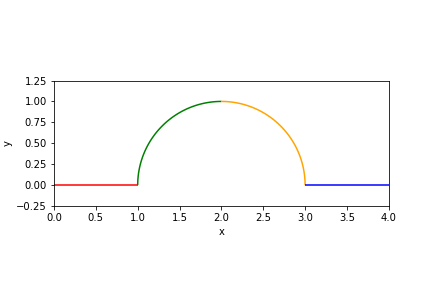
\includegraphics[width=\textwidth]{figures/code/linec_1.png}
        \end{subfigure}
        \begin{subfigure}{0.49\textwidth}
            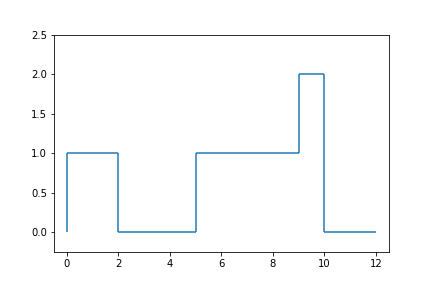
\includegraphics[width=\textwidth]{figures/code/lined_1.png}
        \end{subfigure}
    \end{figure}
\begin{minted}{python}
LineData(FB, edge_table, vertex_table, connect=True)
LineData(FB, edge_table, vertex_table, num_samples=2, connect=False)
\end{minted}
\end{frame}

\begin{frame}{Proposed Work}
\begin{figure}
    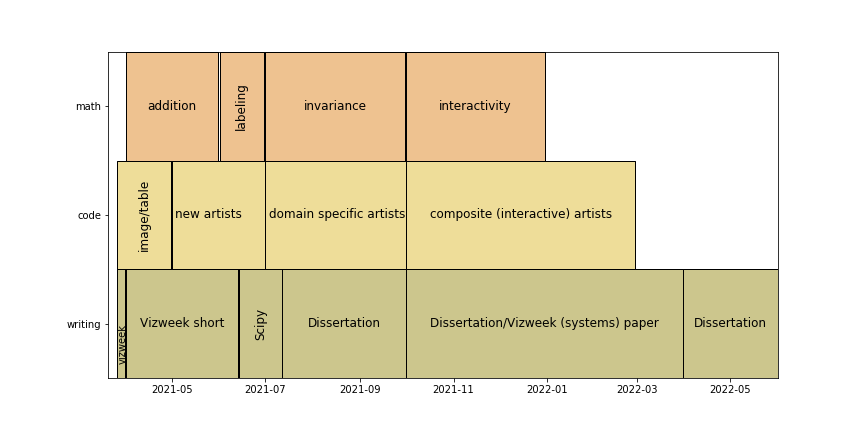
\includegraphics[width=1\textwidth]{figures/intro/gantt.png}
\end{figure}
\end{frame}

\begin{frame}{Acknowledgments}
    \begin{itemize}
        \item Professor Michael Grossberg and Dr. Thomas Caswell
        \item Professor Haralick, Professor Vo, Professor Manovich, Dr. Hanwell
        \item Matplotlib development team 
        \item CZI EOSS (grant number 2019-207333) from the Chan Zuckerberg Initiative DAF, an advised fund of Silicon Valley Community Foundation
    \end{itemize}
    
\end{frame}

\begin{frame}[allowframebreaks]{References}
\printbibliography
\end{frame}
\appendix 

\begin{frame}{Bertin Retinal Variables}
    \begin{figure}
        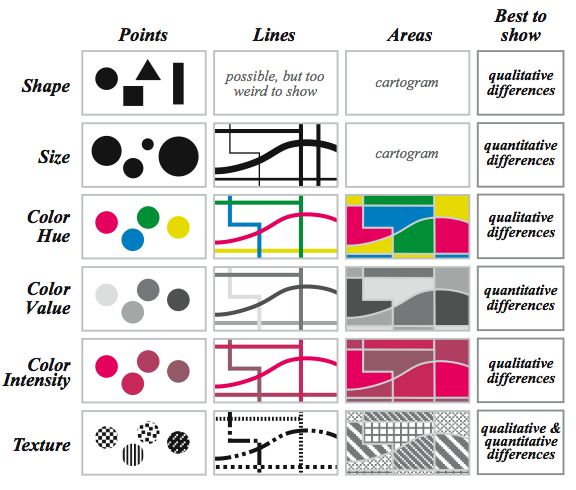
\includegraphics[width=.7\textwidth]{figures/intro/retinal_variables.png}
        \caption{This tabular form of Bertin's retinal variables is from Understanding Graphics \cite{malamedInformationDisplayTips2010} who reproduced it from Krygier and Wood's \textit{Making Maps: A Visual Guide to Map Design for GIS}\cite{krygierMakingMapsVisual2005}}
    \end{figure}
\end{frame}


\begin{frame}{Fiber is all possible values a variable can be \cite{spivakDatabasesAreCategories2010,spivakSIMPLICIALDATABASES}}
    Given a space of all possible values \ftotal\
    \begin{equation*}
        \label{eq:data_types}
        \begin{tikzcd}[ampersand replacement=\&]
            \fttype \arrow[r] \arrow[d, "\pi_{\fsection}"'] \& \ftotal \arrow[d, "\pi"] \\
            \fnames \arrow[r, "\fsection"']                  \& \ftypes       
        \end{tikzcd}
    \end{equation*}
    a fiber component is the restricted space $\ftotal_{\fsection(\fname)}$. 
    \begin{equation*}
        \dfiber = \ftotal_{\fsection(\fname)} = \ftotal_{\ftype} 
    \end{equation*}
    \begin{description}
        \item[\ftypes] data types of the variables in the dataset 
        \item[\ftotal] disjoint union of all values of type $\ftype \in \ftypes$ 
        \item[\fnames] variable names, $\fname \in \fnames$
        \item[\fttype] \ftotal\ restricted to the data type of a named variable   
    \end{description}
\end{frame}

\begin{frame}{Monoid actions}
    A monoid \monoid\ is a set with
    \begin{description}
        \item[associative binary operator] $\ast:\monoid \times \monoid\rightarrow \monoid$
        \item[identity element] $e\in \monoid$ such that $e\ast a= a \ast e = a$ for all $a \in \monoid$. 
    \end{description}
    \begin{block}{left monoid action}
    A set \dfiber\ with an action\cite{nlab:action} $\bullet: \monoid\times \dfiber \rightarrow \dfiber$ with the properties:
        \begin{align*}
            \textbf{associativity}\;& \text{for all } f,g \in \monoid \text{ and } x\in \dfiber,\, f\bullet(g\bullet x) = (f\ast g) \bullet x\\
            \textbf{identity}\;& \text{for all } x\in \dfiber, e\in \monoid,\,  e\bullet x = x 
        \end{align*}
    \end{block}
\end{frame}

\begin{frame}{Keeping track of sections with sheafs}
    Restriction maps of a sheaf describe how local $\iota^*\dsection$ can be glued into larger sections \cite{ghristElementaryAppliedTopology2014,ghristHomologicalAlgebraData2018}
    \begin{equation*}
        \label{eq:sheaf}
        \begin{tikzcd}[ampersand replacement=\&]
            \iota^*\dtotal \arrow[d, "\pi"'] \arrow[r, "\iota^*", hook]             \& \dtotal \arrow[d, "\pi"']                  \\
            U \arrow[r, "\iota", hook] \arrow[u, "\iota^{*}\dsection"', bend right] \& \dbase \arrow[u, "\dsection"', bend right]
        \end{tikzcd}
    \end{equation*}
    The inclusion map $\iota: U \rightarrow \dbase$ pulls \dtotal\ over $U$ such that the pulled back $\iota^*\dsection$ only contains records over $U \subset \dbase$.
\end{frame}

\begin{frame}{Rendering: Define a Pixel}
    \begin{columns}
        \column{0.5\textwidth}
        Given a pixel
        \begin{equation*}
        p=\left[y_{top}, y_{bottom}, x_{right}, x_{left}\right]
        \end{equation*}
        the inverse map of the bounding box 
        \begin{equation*}
        \gbase_{p} ={\gsection_{xy}}^{-1}(p)
        \end{equation*}
        is a region $\gbase_p \subset \gbase$ such that 
        \begin{align}
            \scriptstyle r_p &= \scriptstyle \iint\limits_{S_p} \rho_r(s)ds^{2}\\
            \scriptstyle g_p &= \scriptstyle \iint\limits_{S_p} \rho_g(s)ds^{2}\\
            \scriptstyle  b_p &= \scriptstyle \iint\limits_{S_p} \rho_b(s)ds^{2}
        \end{align}
        yields the color of the pixel. 
        \column{0.5\textwidth}
        \begin{figure}[H]
            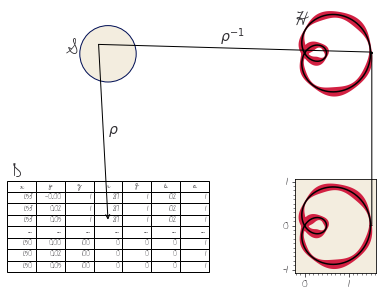
\includegraphics[width=\textwidth]{figures/math/render.png}
        \end{figure}
    \end{columns}
\end{frame}

\begin{frame}{$\mathcal{A}:\mathcal{E}\rightarrow\mathcal{E}$}
    The topological artist is a sheaf map
    \begin{equation*}
    \vartist: \mathcal{O}(\dtotal) \rightarrow \mathcal{O}(\gtotal)
    \end{equation*}
    that carries homomorphism of monoid actions $\varphi: \monoid \rightarrow \monoid^{\prime}$ 
    \cite{cegarraCohomologyMonoidsOperators2019} 
    \begin{equation*}
    \vartist(m\cdot \delement) = \varphi(m)\cdot \vartist(\delement) 
    \end{equation*}
\end{frame}

\begin{frame}{Visual Channel Encoders}
    We define the visual transformers \vchannel\ on components of the data bundle $\dsection_{i}$
    \begin{equation*}
        \label{eq:nu_expanded}
        \{\vchannel_{0}, \ldots, \vchannel_{n}\}: \{\dsection_{0}, \ldots, \dsection_{n}\} \mapsto \{\vsection_{0}, \ldots, \vsection_{n}\}
    \end{equation*}
    as the set of equivariant maps with the constraint 
    \begin{equation*}
        \vchannel_i(m_{\delement}(\dtotal_i)) = \varphi(m_{\delement})(\vchannel_i(\dtotal_i))
    \end{equation*} 
    where $\varphi:\monoid\rightarrow \monoid^{\prime}$ carries a homomorphism of monoid actions. 
\end{frame}

\begin{frame}{\vfiber\ Components}    
\begin{table}[H]
    \renewcommand{\arraystretch}{2}
    \begin{tabulary}{\textwidth}{|l|L|l|}\hline
     $\bm{\vchannel_{i}}$                      & $\bm{\vsection_{i}}$                                                            & $\bm{codomain(\vchannel_{i}) \subset \vfiber_{i}}$  \\ \hline                                              
    position                    & x, y, z, theta, r                                                          & $\mathbb{R}$   \\ \hline
    size                        & linewidth, markersize                                            & $\mathbb{R}^{+}$   \\ \hline
    shape                       & markerstyle                                                      & $\{f_{0}, \ldots, f_{n}\}$ \\ \hline
    color                       & color, facecolor, markerfacecolor, edgecolor  & $\mathbb{R}^{4}$ \\ \hline
    \multirow{2}{*}{texture}    & hatch                                                            & $\mathbb{N}^{10}$\\\cline{2-3}
                                & linestyle                                                        & $(\mathbb{R}, \mathbb{R^+}^{n, n\%2=0})$ \\ \hline              
    \end{tabulary}
    \label{tab:mpl_visual_variable_fiber}
\end{table}
\end{frame}
\begin{frame}{Monoid Equivariance: Partial Orders}
    \begin{figure} %break out steps/reveal
        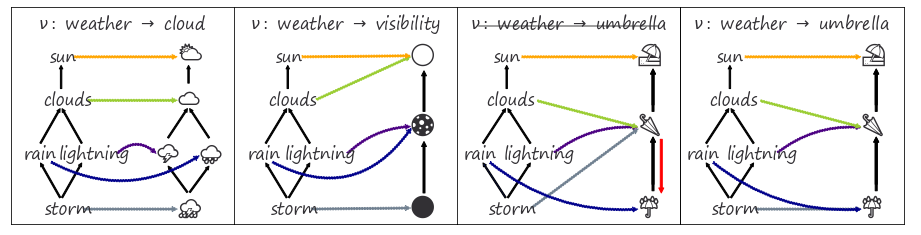
\includegraphics[width=1\textwidth]{figures/math/monoid_equivariant.png}
    \end{figure}
\end{frame}

\begin{frame}{Glyph}
    The glyph is the graphic generated by $\vmark(\gbase_{\dbasepathpoint})$ where the path connected components $\dbasepath \subset \dbase$ are defined 
    \begin{equation*}
    \dbasepath = \{\dbasepathpoint \in \dbase \text{ s. t. } \exists \gamma \text{ s.t. } \gamma(0)=\dbasepoint \text{ and }\gamma(1)=\dbasepathpoint\}
    \end{equation*}
    such that the  path $\gamma$ from \dbasepoint\ to \dbasepathpoint\ is a continuous function from the interval [0,1] and $\gbase_{\dbasepathpoint}$ is the region
    \begin{equation*}
        \begin{tikzcd}[ampersand replacement=\&]
            \gtotal \arrow[r, shift left] \& \gbase_\dbasepathpoint \arrow[rr, "\vindex(\gbasepoint)", shift left] \arrow[l, "\gsection(\gbase_\dbasepathpoint)"] \& \& \dbasepath_{\dbasepoint} \arrow[ll, "\vindex^{-1}(\dbasepath)"]
            \end{tikzcd}
        \label{eq:mark}
    \end{equation*}
    such that the glyph is differentiable, in keeping with Ziemkiewicz and Kosara's description of a glyph\cite{ziemkiewiczEmbeddingInformationVisualization2009}.
\end{frame}

\begin{frame}{Artist Equivalance class}
    When artists share a base space 
    \begin{equation*}
        \dbase_2 \hookrightarrow \dbase_1
    \end{equation*}
    a composition operator can be defined such that the the artists can be considered to be acting on different components of the same section. 
\end{frame}

\begin{frame}[fragile]{Complex \vchannel}
    \begin{minted}{python}
    class Categorical:
        def __init__(self, mapping):
            # check that the conversion is to valid colors
            assert(mcolors.is_color_like(color) for color in mapping.values())
            self._mapping = mapping
    
        def __call__(self, value):
            # convert value to a color
            return [mcolors.to_rgba(self._mapping[v]) for v in values]
    \end{minted}
    That we can test for action equivariance
    \begin{minted}{python}
    def test_nominal(values, encoder):
        m1 = list(zip(values, encoder(values)))
        random.shuffle(values)
        m2 = list(zip(values, encoder(values)))
        assert sorted(m1) == sorted(m2)
    \end{minted}
\end{frame}

\begin{frame}[fragile]{Artist}
    \begin{minted}{python}
        class ArtistClass(matplotlib.artist.Artist):
            def __init__(self, data, transforms, *args, **kwargs):
                # properties that are specific to the graphic
                self.data = data 
                self.transforms = transforms
                super().__init__(*args, **kwargs)
        
            def assemble(self, **args):
                # set the properties of the graphic
        
            def draw(self, renderer):
                # returns K, indexed on fiber then key 
                view = self.data.view(self.axes) 
                # visual channel encoding applied fiberwise 
                visual = {p: t['encoder'](view[t['name']])
                          for p, t in self.transforms.items()}
                self.assemble(**visual)
                # pass configurations off to the renderer
                super().draw(renderer)
        \end{minted}
\end{frame}


\begin{frame}[fragile]{Artists: Scatter \& Line}
\begin{minted}{python}
class Point(mcollections.Collection):
    def assemble(self, x, y, s, facecolors='C0' ):
        # construct geometries of the circle glyphs in visual coordinates
        self._paths = [mpath.Path.circle(center=(xi,yi), radius=si) 
                    for (xi, yi, si) in zip(x, y, s)] 
        # set attributes of glyphs, these are vectorized 
        # circles and facecolors are lists of the same size
        self.set_facecolors(facecolors)

class Line(mcollections.LineCollection):
    def assemble(self, x, y, color='C0'):
        #assemble line marks as set of segments 
        segments = [np.vstack((vx, vy)).T for vx, vy in zip(x, y)]
        self.set_segments(segments)
        self.set_color(color)
\end{minted}
\end{frame}


\begin{frame}[fragile]{View}
\begin{minted}{python}
def view(self, axes):
    table = defaultdict(list)
    for k in self.keys:
        table['index'].append(k)
        for (name, value) in zip(self.FB.fiber.keys(), self.tau(k)[1]):
            table[name].append(value)
    return table
\end{minted}
\begin{description}
    \item [\mintinline{python}{VertexSimplex}] (name, value), value is scaler
    \item [\mintinline{python}{EdgeSimplex}]  (name, value), value is [x0, ..., xn]
\end{description}
\end{frame}

\begin{frame}[fragile]{Fiber Bundle}
    \begin{minted}{python}
    @dataclass
    class FiberBundle:
    """
    Attributes
    ----------
    K: {'tables': []}
    F: {variable name: type}
    """
        K: dict 
        F: dict
    \end{minted}
\end{frame}

\begin{frame}[fragile]{GraphLine Data Model}
\begin{minted}{python}
class GraphLine:
    def __init__(self, FB, edge_table, vertex_table, num_samples=1000,
                        connect=False):
        #set args as attributes and generate distance
        if connect: # test connectivity if edges are continuous
            assert edge_table.keys() == self.FB.F.keys()
            assert is_continuous(vertex_table)

    def tau(self, k):
        # evaluates functions defined in edge table
        return(k, (self.edges[c][k](self.distances) 
                        for c in self.FB.F.keys()))

    def view(self, axes):
        # walk the edge_vertex table to return the edge function
        table = defaultdict(list)
        for (i, (start, end)) in sorted(zip(self.ids, self.vertices), 
                                            key=lambda v:v[1][0]):
            table['index'].append(i)
            # same as view for line, returns nested list
            for (name, value) in zip(self.FB.F.keys(), self.tau(i)[1]):
                table[name].append(value)
        return table
\end{minted}
\end{frame}
\end{comment}